\section{Unreachable Regions for Automorphic Transforms}
\begin{multicols}{2}
\label{sec:un}
Before we focus on the area of good filters, let us study the area of 
available filters.
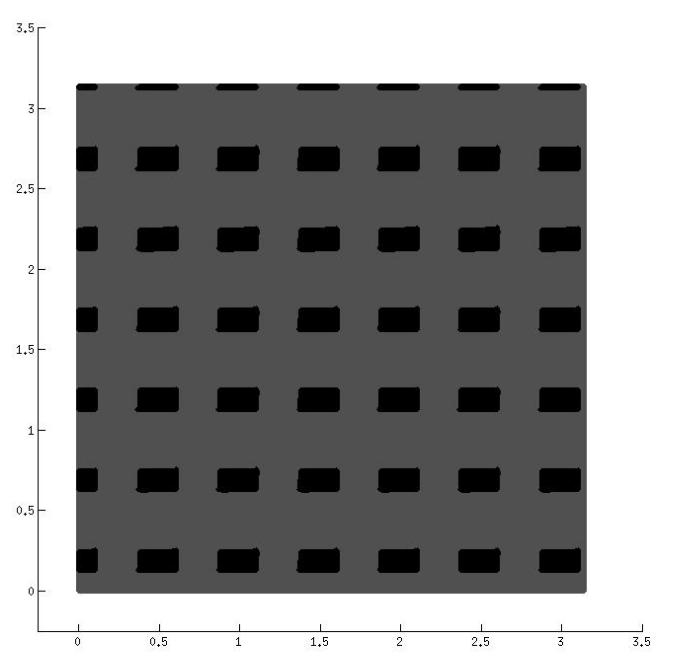
\includegraphics[width=0.5\textwidth]{theta_s_in_uns.jpg}
Now, for a quadratic polynomial, the coefficients corresponding to
complex roots lie within a parabola. This is easily established, 
since, for complex roots of a monic polynomial 
$P(\lambda) = \lambda^2 + x\lambda + y$, we must have
$x^2 - 4y < 0$. Whether an eigenvalue is complex or not is not of
much importance. But for this system of matrices, and indeed it seems for
most such systems, there appear to be regions inaccessible via 
automorphic \glspl{spe}. And, in the 2-dimensional case, such 
regions seem to share two common properties: 
\begin{enumerate}
\item They are conic sections;
\item They lie within this parabola.
\end{enumerate}
For certain systems, for example the system in the previous example,
the entire parabola is inaccessible. A plot of the corresponding
eigenvalues reveals that these inaccessible regions have their 
analogues in the eigenspace. For the present system, since the entire
parabola was inaccessible by automorphic transforms, eigenvalues of all
stable filters are necessarily real.
\begin{figure*}
\centering
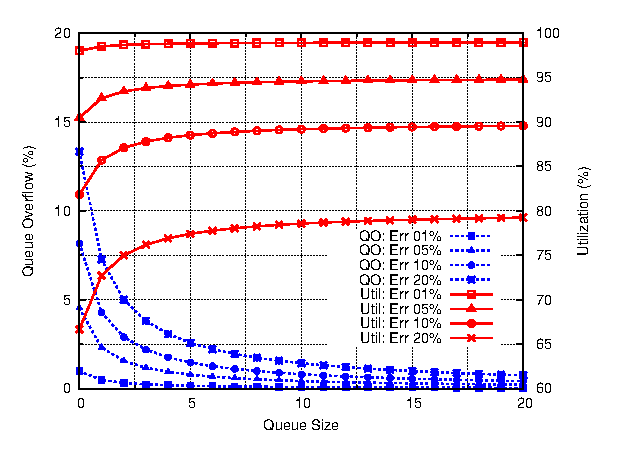
\includegraphics[width=0.9\textwidth]{qsize-util-err.eps}
\caption{Good CPCs (shown in black) and reachable CPCs of a 2D system}
\label{fig:s_vs_us}
\end{figure*}

These special areas also exist for the 3-dimensional case, and
presumably for all dimensions. In the 3-dimensional case, contrary 
to what one might expect, these regions are not cones or
revolutions of conic sections, but have quite arbitrary shapes, with 
symmetry a common feature in the cases examined so far.
The high number of variables involved have made analytical derivation 
of the equations of these regions very difficult. One way to do it 
numerically would be to evaluate the Jacobian at each point. Anywhere 
outside the unreachable region, a point can move in any direction. 
However, at the surface of the region, the point is constrained from 
moving further within the region. Thus the derivative of the 
coordinate vector along these directions would be zero. Hence the 
Jacobian would be rank-deficient, and its determinant would be zero.
This is true independent of the basis chosen for obtaining the Jacobian.
Thus, but determining where the Jacobian is zero, one can approximate 
the surface of the unreachable region.

This method was applied to the present example. For evaluating the partial 
derivatives that make up the Jacobian, a first-order finite difference 
method was used. Then a root-finding algorithm was applied on the Jacobian 
determinant for each grid line. The resultant boundary points are shown in 
\autoref{fig:bound}. The fit (quadratic) is reasonably accurate, as can be 
inferred from the figure. The extra points are due to the gaps in 
calculated points, which arise due to the uniform intervals in which 
the range of values of \gls{t} was divided. The bottom edge, and some 
of the gaps in the space of stable points, which may or may not be 
unreachable, were also detected by this method.
%
\begin{figure*}
\centering
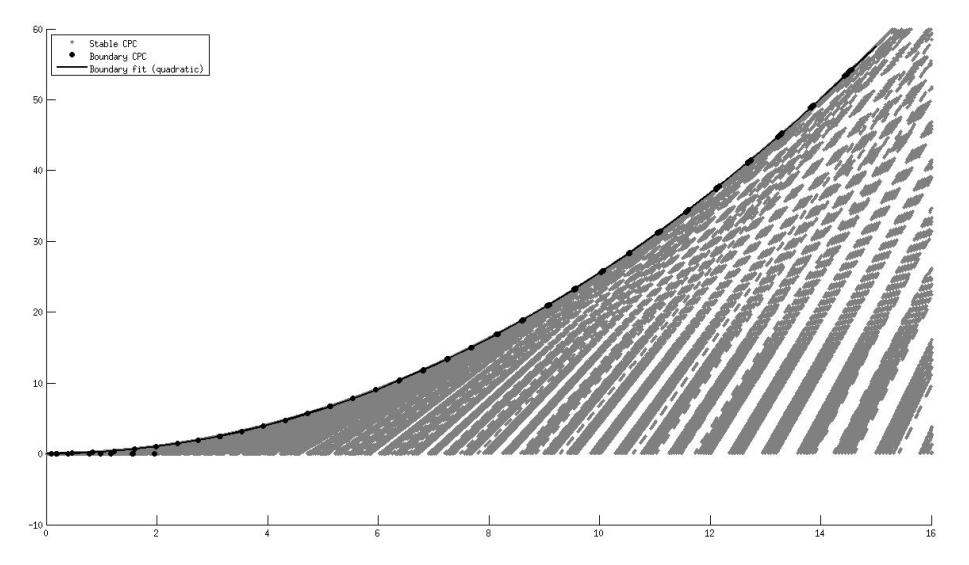
\includegraphics[width=0.9\textwidth]{bound.jpg}
\caption{Scatter of $(\theta_1, \theta_2)$ for good CPCs (in black) over reachable CPCs}
\label{fig:theta}
\end{figure*}
%
\reversemarginpar
\begin{figure*}
\centering
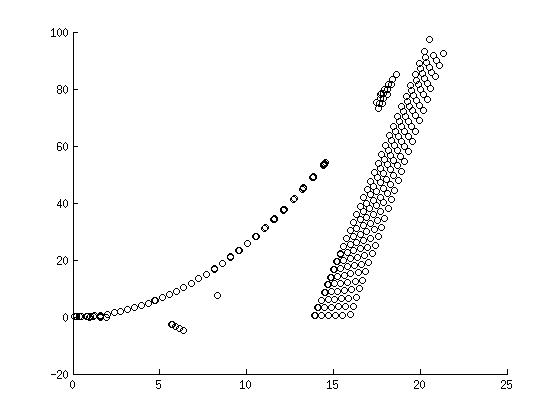
\includegraphics[width=0.9\textwidth]{allbound.jpg}
\caption{Calculated boundary points of unreachable CPC region}
\marginnote{These figures are inside a multicolumn area (using the multicol package. \
So technically, \textsc{technically}, I have satisfied the requirement of having \
a figure span both columns.}
\label{fig:bound}
\end{figure*}
%
\begin{figure*}
\centering
\subfloat[A 3D scatter, seemingly random]{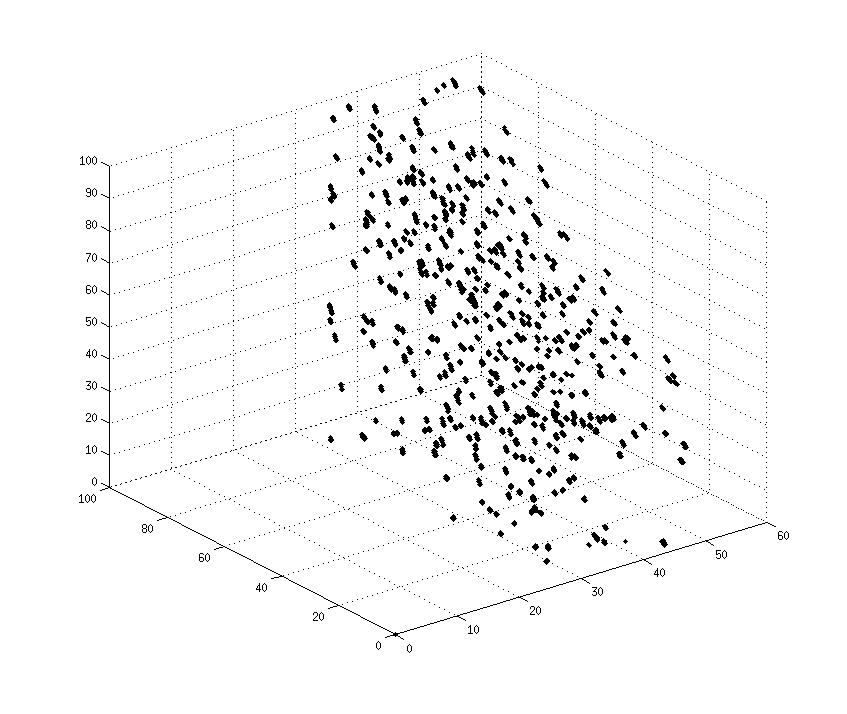
\includegraphics[width=0.48\textwidth]{3d.jpg}}
\subfloat[Projection on the x-y plane, revealing a pattern.]{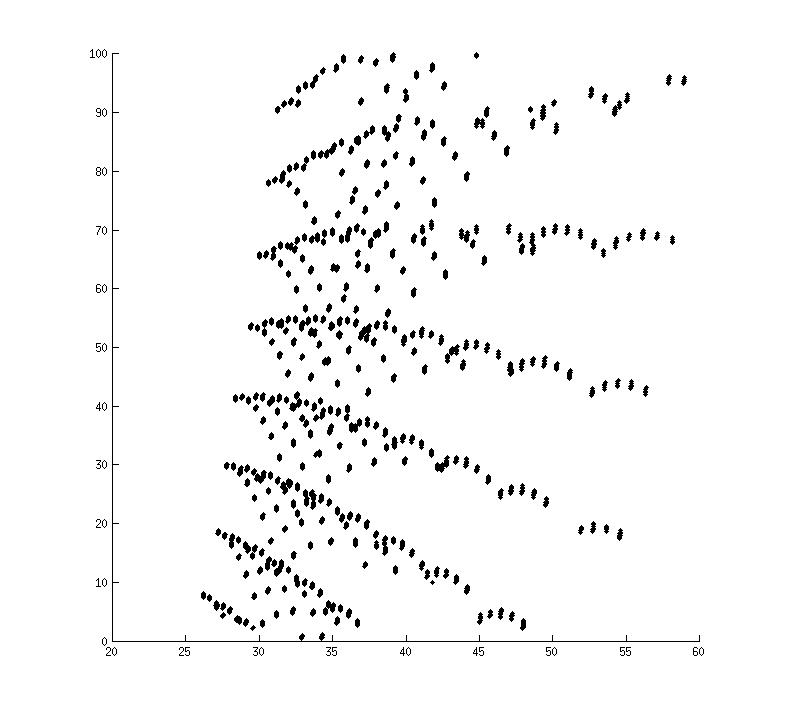
\includegraphics[width=0.48\textwidth]{3d2.jpg}}
\caption{Good CPCs for a 3D system}
\label{fig:3d}
\end{figure*}
\end{multicols}
